% ===================================================================
%  Das Vokaltrapez der IPA mit TikZ – deutsche Vokale hervorgehoben
%  Kompilieren: pdflatex vorlage_vokaltrapez.tex
% ===================================================================
\documentclass[border=0.1mm]{standalone}
\usepackage[T1]{fontenc}
\usepackage{lmodern}
\usepackage{amsmath}
\usepackage{amssymb}
\usepackage[safe]{tipa}
\usepackage{tikz}
\usetikzlibrary{arrows.meta}

\definecolor{akzentblau}{HTML}{2563EB}

\begin{document}
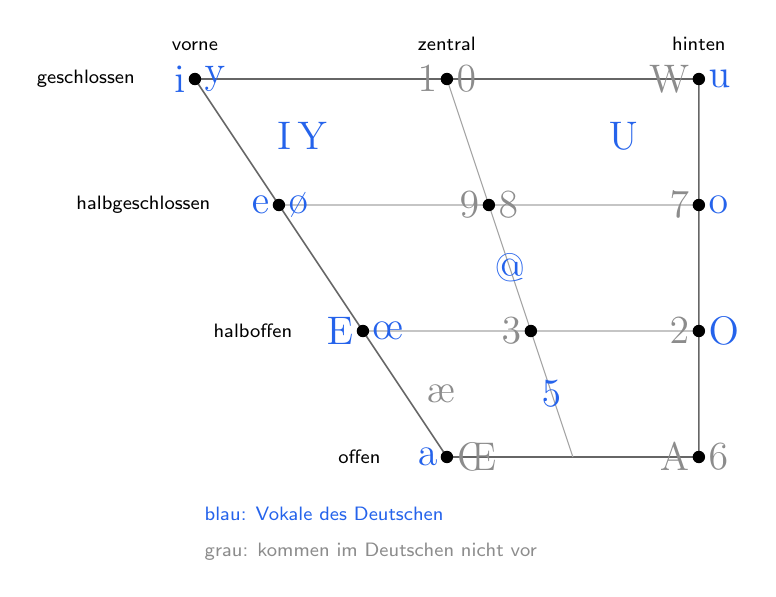
\begin{tikzpicture}[scale=1.6, font=\sffamily\scriptsize]
  % --- Das Trapez: oben 4 breit, unten 2 breit, 3 hoch ---------------
  % linke Kante: x = 2 - 2y/3,  Mittellinie: x = 3 - y/3,  rechts: x = 4
  \draw[black!60, line width=0.6pt] (0,3) -- (4,3) -- (4,0) -- (2,0) -- cycle;
  \draw[black!35] (2/3,2) -- (4,2)  (4/3,1) -- (4,1)  (2,3) -- (3,0);

  % --- Beschriftung der Achsen ----------------------------------------
  \node[above] at (0,3.15) {vorne};
  \node[above] at (2,3.15) {zentral};
  \node[above] at (4,3.15) {hinten};
  \node[left] at (-0.4,3)   {geschlossen};
  \node[left] at (0.2,2)    {halbgeschlossen};
  \node[left] at (0.85,1)   {halboffen};
  \node[left] at (1.55,0)   {offen};

  % --- Vokale: \vokal{x}{y}{ungerundet}{gerundet}{Farbe links}{Farbe rechts}
  %     links vom Punkt ungerundet, rechts gerundet
  \newcommand\vokal[6]{
    \fill (#1,#2) circle (1.4pt);
    \node[left,  font=\Large, text=#5] at (#1,#2) {\textipa{#3}};
    \node[right, font=\Large, text=#6] at (#1,#2) {\textipa{#4}};
  }
  \colorlet{de}{akzentblau}      % kommt im Deutschen vor
  \colorlet{nd}{black!45}     % kommt im Deutschen nicht vor

  \vokal{0}{3}{i}{y}{de}{de}               % geschlossen
  \vokal{2}{3}{1}{0}{nd}{nd}
  \vokal{4}{3}{W}{u}{nd}{de}
  \vokal{2/3}{2}{e}{\o}{de}{de}            % halbgeschlossen
  \vokal{7/3}{2}{9}{8}{nd}{nd}
  \vokal{4}{2}{7}{o}{nd}{de}
  \vokal{4/3}{1}{E}{\oe}{de}{de}           % halboffen
  \vokal{8/3}{1}{3}{\textcloserevepsilon}{nd}{nd}
  \vokal{4}{1}{2}{O}{nd}{de}
  \vokal{2}{0}{a}{\OE}{de}{nd}             % offen
  \vokal{4}{0}{A}{6}{nd}{nd}

  % Vokale zwischen den Linien (ohne Punkt)
  \node[font=\Large, text=de] at (0.85,2.55) {\textipa{I\,Y}};
  \node[font=\Large, text=de] at (3.4,2.55) {\textipa{U}};
  \node[font=\Large, text=de] at (2.5,1.5)  {\textipa{@}};
  \node[font=\Large, text=nd] at (1.95,0.5) {\textipa{\ae}};
  \node[font=\Large, text=de] at (2.83,0.5) {\textipa{5}};

  % --- Legende ---------------------------------------------------------
  \node[anchor=west, text=de] at (0,-0.45) {blau: Vokale des Deutschen};
  \node[anchor=west, text=nd] at (0,-0.75) {grau: kommen im Deutschen nicht vor};
\end{tikzpicture}
\end{document}
